% 2004_fujian_science_q19_fig1: tetrahedron S-ABC, M midpoint of AB, N midpoint of SB.
% Solid visible outline: S-A, S-B, A-B, M-N. All edges incident to C dashed.
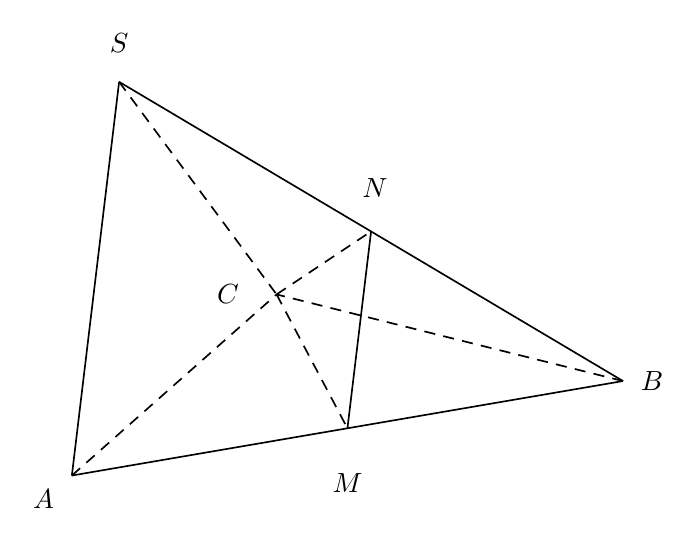
\begin{tikzpicture}[x=1cm,y=1cm,font=\normalsize,
  solidedge/.style={solid,line width=.6pt},
  dashedege/.style={dashed,line width=.6pt,dash pattern=on 4pt off 3pt},
  geomlabel/.style={font=\normalsize,inner sep=2pt}]
\coordinate (S) at (0.6,5);
\coordinate (A) at (0,0);
\coordinate (B) at (7,1.2);
\coordinate (C) at (2.6,2.3);
\coordinate (M) at (3.5,0.6);
\coordinate (N) at (3.8,3.1);
% hidden edges through C
\draw[dashedege] (S)--(C);
\draw[dashedege] (A)--(C);
\draw[dashedege] (B)--(C);
\draw[dashedege] (C)--(M);
\draw[dashedege] (C)--(N);
% visible outline
\draw[solidedge] (S)--(A);
\draw[solidedge] (S)--(B);
\draw[solidedge] (A)--(B);
\draw[solidedge] (M)--(N);
\node[geomlabel,above] at (0.6,5.3) {$S$};
\node[geomlabel,below left] at (-0.15,-0.1) {$A$};
\node[geomlabel,right] at (7.15,1.2) {$B$};
\node[geomlabel,left] at (2.2,2.3) {$C$};
\node[geomlabel,below] at (3.5,0.1) {$M$};
\node[geomlabel,above] at (3.85,3.45) {$N$};
\end{tikzpicture}
